\subsubsection{Dynamik der Drehbewegung}
\begin{itemize}
	\item Zentripetalkraft (Ursache für Zentralbewegung) und Zentrifugalkraft (Fliehkraft) sind gleich gross, aber entgegengerichtet.
	\item Trägheitsmoment: Bei einem drehbaren Körper ist das Verhältnis von wirkendem Drehmoment zur erzielten Winkelbeschleunigung eine konstante Grösse, dem Trägheitsmoment.
\end{itemize}
\begin{tabbing}
	\begin{tabu} to \linewidth {X l X l}
		\toprule
		Trägheitsmoment & $J = r^2\Delta m$ &
		Trägheitsmoment & $J = \sum_{i=1}^{n}r_i^2 \Delta m_i$ \\
		Zentripetalkraft & $F_r = F_z = \frac{mv^2}{r} = m\omega^2r = p\omega$ & 
		Zentripetalbeschl & $a_r = a_z = r \omega^2 = \frac{v^2}{r}$ \\
		Rotationsleistung & $P = M \omega$ &
		Rotationenergie & $E_{rot} = \frac{J\omega^2}{2}$\\
		Drehmoment & $M = J\alpha$ &
		Rotationsarbeit & $W = M\varphi$ \\
		Drehimpuls & $L = J \omega = M \cdot t = r\cdot p$ & 
		Drehimpuls einer Punktmasse & $\Delta M = \frac{\Delta L}{\Delta t}$ \\
	\end{tabu}
\end{tabbing}

\begin{tabbing}
	\begin{tabu} to \linewidth {l X l}
		Variable & Bedeutung & SI-Einheit \\
		\midrule
		$J$ & Trägheitsmoment & $J = kg \cdot m^2$ \\ 
		$m$ & Masse eines dünnen Kreisringes (Umfang) & $kg$ \\ 
		$r$ & einheitlicher Abstand aller Massenelemente von der Drehachse & $m$ \\ 
		$m_i$ & Massenelement & $kg$\\ 
		$P$ & Leistung & $W$ \\ 
		$p$ & Impuls des Körpers & $N \cdot s$ \\
		$M$ & Drehmoment, das die Drehung verursacht & $N \cdot m$ \\ 
		$\omega$ & Winkelgeschwindigkeit des Körpers & $\frac{rad}{s} = \frac{1}{s}$ \\ 
		$L$ & Drehimpuls des rotierenden Körpers & $\frac{kg \cdot m^2}{s} = N \cdot m \cdot s$  \\ 
		$\alpha$ & Winkelbeschleunigung & $\frac{rad}{s^2} = \frac{1}{s^2}$ \\
		\bottomrule
	\end{tabu}
\end{tabbing}



\begin{minipage}[h!]{0.5\linewidth}
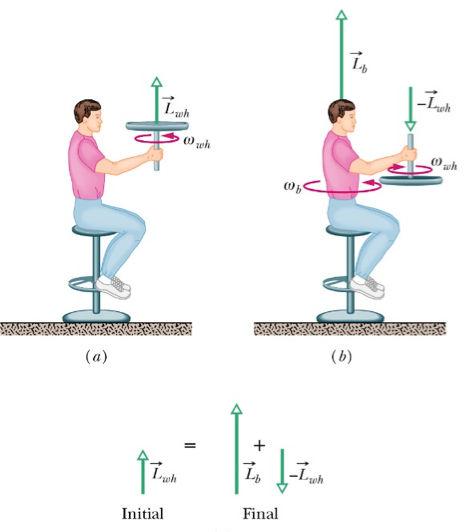
\includegraphics[width=0.8\linewidth]{images/drehimpuls}
\end{minipage}
\hfill
\begin{minipage}[h!]{0.5\linewidth}
	\begin{align*}
		L_b &= J_b \omega_b \\
		L_{wh} &= J_{wh} \omega_{wh} \\
		L_{wh} &= L_b - L_{wh} \\
		J_{wh} \omega_{wh} &= J_b \omega_b - J_{wg} \omega_{wg} \\
		\omega_b &= \frac{2J_{wh}}{J_b} \omega_{wg} \\
	\end{align*}
\end{minipage}